\chapter{Competitor Rules}

\section{Safety}

\oldrule{6.3}
No safety gear is needed.

\section{Unicycles}

\oldrule{6.31.3}
One standard unicycle only (see definition).
No brakes or handlebars.
There are no limitations on wheel or crank arm size.

\section{Rider Identification}
\section{Protests}

\oldrule{6.9}
Must be filed in writing, within 15 minutes from the posting of event results.
Protest against judges' scores is not permissible.
Protest is only possible against calculation mistakes or other mistakes not connected to the scoring.
The Chief Judge must resolve all protests within 30 minutes from receipt of the written form.

\section{Deadline For Signing Up}

\section{Event Flow}

\subsection{Riders Must Be Ready}

\oldrule{6.2.1}
Riders who are not ready at their scheduled performance time may or may not be allowed to perform after the last competitor in their age group or category.
The Chief Judge will remember to consider language barriers, and that riders may be engaged in convention work to slow them down.
Except for Standard Skill, a rider may not perform before a different set of judges than those that judged the rest of their age group or category.

\subsection{Time Limits}
\oldrule{6.31.2}
Three minutes (all ages).

\subsection{Judging Method}
\oldrule{6.31.6}
Riders are judged only on the quality of execution of the skills they have chosen to perform.
Each figure has a predetermined point value.
Judges deduct points for mistakes, such as dismounts, poor form, performing figures out of order, etc.

\subsection{Music}
\oldrule{6.31.4}
Music is not judged.
Background music may be provided during routines or competitors may provide their own.
Competitors may also, at their request, have no music played.
See also section \ref{sec:freestyle_music}.

\subsection{Costume and Props}
\oldrule{6.31.5}
Clothing has no influence on the score.
Riders are encouraged to dress in the uniform of their national teams or clubs, or in clothing that represents their teams, groups or countries.
No props.

\subsection{Skills to be Performed}
\oldrule{6.31.7}
Only skills found in the IUF Standard Skill List may be used.
The proper methods for performing these skills are found in the `Descriptions' section of this list.
If illustrations of figures disagree with their descriptions, the descriptions apply.

\section{Rider's No-Signal Option \label{sec:freestyle_riders-no-signal-option}}

\oldrule{6.35.1}
If a rider provides their own music and wants acoustic signals, they must indicate this when they sign up with the Rider Liaison.
If a rider does not provide their own music, acoustic signals will automatically be used unless the rider requests ``No acoustic signals'' when signing up with the Rider Liaison.
If no acoustic signals, there will not be a `Start' signal or the 1-minute and 2-minute signals.
In all situations, the Timer will still keep the time, and if the rider exceeds the time limit, the Timer will make the `double acoustic signal' to indicate the rider has run overtime.

\section{Floor, Markings And Figure Shapes}
\oldrule{6.36}
See diagram.
The riding surface must allow flawless riding.
The riding area must be sufficiently illuminated.
An IUF representative will inspect the area to make sure it conforms to the requirements, and declare it ridable.
The surface of the riding floor must be clean, level, smooth and shall not be slippery.
Competition can be held on a floor that has not been declared ridable by the panel, but the results of such competition may not be officially recognized by the IUF, after investigation by the IUF rules committee.

\subsection{Riding Area Boundaries \label{subsec:freestyle_floor-markings-figure-shapes_riding-area-boundaries}}
\oldrule{6.36.1}
For international competitions, the outer boundaries must be 11 x 14 meters.
For other competitions, if space does not permit, the size may be smaller but will be no less than 9 x 12 meters.
All lines must be at least 3 cm wide and clearly marked, including the outer boundaries.

\begin{figure}[h]
\begin{center}
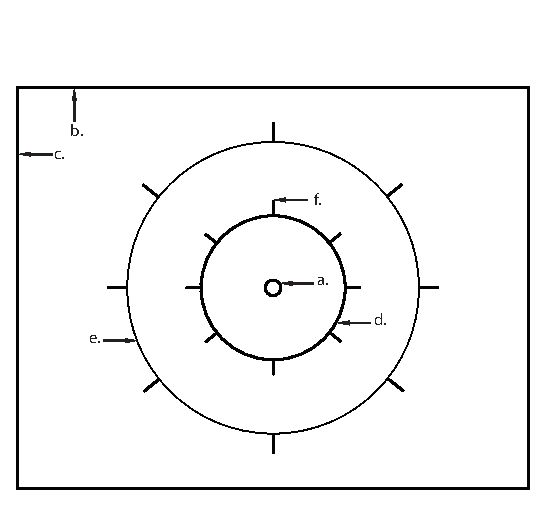
\includegraphics{std_skill_pattern_labeled}
\end{center}
\vspace{-20pt}
\caption{Riding Area Boundaries \label{fig:std_skill_pattern_labeled}}
\vspace{-10pt}
\end{figure}

\begin{enumerate}[a.]
\item Center circle (50 cm diameter)
\item Long edge of riding area (faces judges)
\item Short edge of riding area
\item Inner circle (4 m diameter) for circle figures
\item Outer circle (8 m diameter) for line and figure eights.
\item Quarter and diagonal circle marks (length 1 m) on the 4 m and 8 m circles.
Diagonals marked by going from corner to corner of the riding boundary.
\end{enumerate}

\subsection{Line Figure}
\oldrule{6.36.2}
\begin{wrapfigure}{r}{0.35\textwidth}
\vspace{-35pt}
\begin{center}
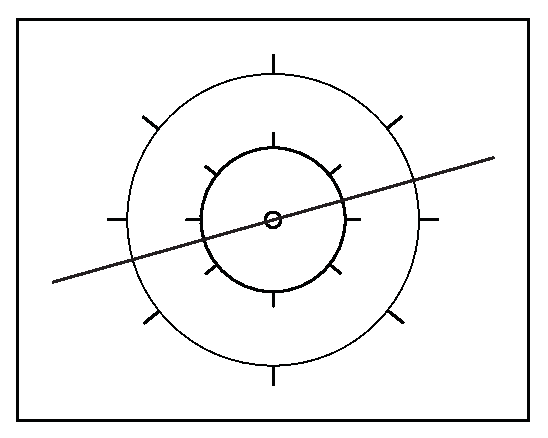
\includegraphics[width=0.33\textwidth]{std_skill_line_figure}
\end{center}
\vspace{-20pt}
\caption{Line Figure\label{fig:std_skill_line_figure}}
\vspace{-10pt}
\end{wrapfigure}
Lines, circles and figure eights may be ridden in any direction.
Line figures start outside the large (8 m) circle, cross the center circle, and continue outside the large circle.
The rider must be in position for the figure before the hub crosses over the outside edge of the line.
For seat drag figures where the seat is forward of the riding direction, the rider must be in position before the seat crosses the outside edge of the line.
The line should be straight.
Circles and figure eights can be started at any point, as long as the rider completes the figure by crossing over the starting point.

\subsection{Circle Figure}
\oldrule{6.36.3}
\begin{wrapfigure}{r}{0.35\textwidth}
\vspace{-75pt}
\begin{center}
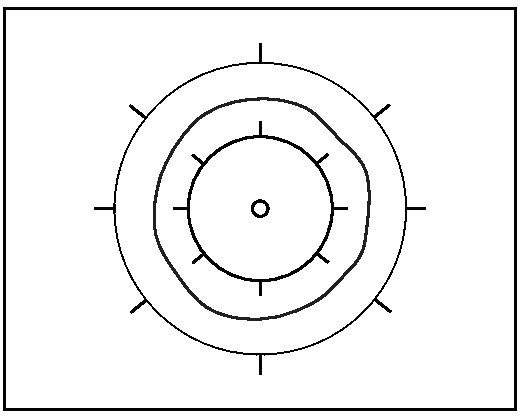
\includegraphics[width=0.33\textwidth]{std_skill_circle_figure}
\end{center}
\vspace{-20pt}
\caption{Circle Figure\label{fig:std_skill_circle_figure}}
\vspace{-10pt}
\end{wrapfigure}
Circle figures are ridden in the area between the 4 m and 8 m circle lines.
If the rider crosses the 4 m line while performing the figure, the circle must be restarted from the point where the rider re-crosses to the outside of the 4 m circle.
Crossing the 8 m line does not invalidate the figure.
Circle figures should be as round as possible.

\subsection{Figure Eight}
\oldrule{6.36.4}
\begin{wrapfigure}{r}{0.35\textwidth}
\vspace{-45pt}
\begin{center}
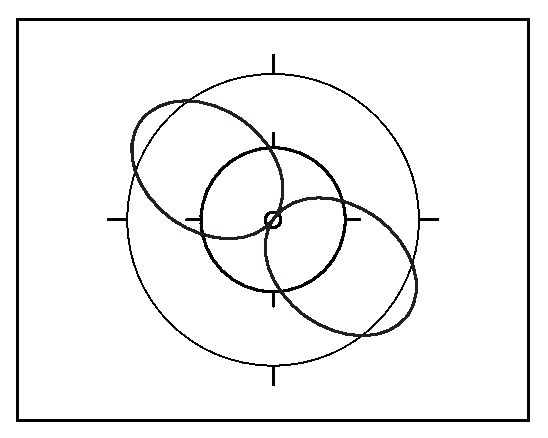
\includegraphics[width=0.33\textwidth]{std_skill_figure_eight}
\end{center}
\vspace{-20pt}
\caption{Figure Eight\label{fig:std_skill_figure_eight}}
\vspace{-10pt}
\end{wrapfigure}
The two circles making up the 8 should be the same size, and the orientation of the 8 can be in any direction.
The rider must pass outside the 8 m circle on each end of the 8, and cross the center circle at the middle.
The two halves of the figure 8 must be circular, with diameters of at least 4 m.

\section{Mounts, Transitions, Axis, Single And Counted Short Skills}

\oldrule{6.37}
These are all collectively called ``non-riding skills''.
May be performed anywhere in the riding area unless stated differently in the description.

\section{Body Form}
\oldrule{6.38}
Unless otherwise noted, each figure must be performed with riders sitting up straight with their arms stretched and horizontal.
Hands must be flat with palms down and fingers together.
Arms do not have to be straight out to the sides.
As long as arms are outstretched and horizontal, they may point in any direction.

\section{Dismounts}
\oldrule{6.39}
All dismounts must be controlled, including the dismount at the end of the routine.
A controlled (intentional) dismount is where the rider comes to a stop and steps off the unicycle.
Dismounts executed otherwise will be considered unintentional.
A dismount occurs any time a rider touches the floor, except in skills where the rider is required to touch the floor, or when a foot on a pedal touches the floor.
The rules demand that the rider dismounts in a sportsmanlike manner at the end of the routine.
Failure to do so will result in a wave for insecure exit.

\section{Assisting Riders}
\oldrule{6.40}

At international events it is forbidden for a rider to get verbal assistance or helping gestures from a person outside the riding area, since this is interference with the rider by an outside person.
At international events it is forbidden for a rider to use any props (including people) during the 3-minute routine.
Any competitor caught getting assistance (verbal or nonverbal) or using props may be disqualified from the competition.
Also, a rider may not look at the list of skills while performing the routine.
This includes skills written on the competitor's hand, a piece of paper or elsewhere.
Each occurrence of a competitor looking at a skills list will result in a wave.

\section{Standard Skill Judging Sheet}
\oldrule{6.41}
Before competing in Standard Skill, each rider must fill out and turn in a judging sheet listing his or her routine.
This list includes the number, name, and point value of each figure to be performed in the routine, in the order in which they will be ridden.

\subsection{Skills To Be Used}
\oldrule{6.41.1}
The maximum number of figures allowed is 18.
Of those 18 figures, no more than 12 may be other than a riding skill.
Skills with numbers 101 and higher are limited to a maximum of 12.
If a rider only chooses 12 skills for the whole routine, it is allowed for all of these to be non-riding skills.

\textbf{Note:} Each figure number may appear only once on the judging sheet.
This means that, for example, if a rider uses figure 15 b, he or she may not use 15 a, c, d, e, f, g, or h.

\subsection{Skill Order}
\oldrule{6.41.2}

The 18 figures must be performed in the exact same order as they appear on the judging sheet.
Figures left out according to their order on the judging sheet will be devaluated 100\%.
This devaluation remains, even if the figure is performed later in the routine.
\textbf{Example:} The skills on a judging sheet are: wheel walk, one-foot, idle, riding backwards.
The rider does the wheel walk, skips the one-foot and idle, then performs the riding backwards, followed by the one-foot and the idle.
The technical judge will mark both the 1-ft and idle with a 100\% devaluation.

\subsection{Filling Out Judging Sheet}
\oldrule{6.41.3}

The completed judging sheet must be sent in before the deadline date set by competition organizers.
When filling out the sheet, each figure name must be written out exactly as it appears on the Standard Skill List, with no further abbreviations.
Figure numbers, letters, and point values must be included, and the total Difficulty score (total points for all figures in the routine) must be filled in.
The judges have to check the judging sheets and, if possible in contact with the competitor, correct any mistakes.
Any disadvantage resulting from filling out a judging sheet incorrectly will be at the competitor's expense, and will not be valid grounds for protest.
Judging sheets, once checked and approved for competition, cannot be changed.


\subsection{Start Of Performance}

\oldrule{6.33.1}
The judging begins when the timer blows a one second whistle signifying the beginning of the three minute routine or when a predetermined piece of music begins; the stopwatch will begin timing immediately following the one second acoustic signal or music.
The end of each minute will be indicated by acoustic signals.
This may be made optional as described in section \ref{sec:freestyle_riders-no-signal-option}.
A final one-second acoustic signal will signify the completion of the three-minute allotment.

\subsection{End Of Performance}
\oldrule{6.34.1}
In Standard Skill, if the rider is in mid-figure, only the part of that figure that was executed before the time ended will be counted (see section \ref{subsec:freestyle_difficulty-devaluations_skill-completion}).
If the figure was less than 50\% complete, a 100\% devaluation will be given.
If between 50\% and 100\% was completed, a 50\% devaluation will be given.
Any figures that have not been performed receive 100\% devaluations.
